% ============================================================================
% NEWSLETTER — Development & Deployment of the GMFM Assessment Application
% for Cerebral Palsy Assessment
% Compile with: xelatex newsletter.tex  (required for Times New Roman)
% ============================================================================
\documentclass[11pt,a4paper]{article}

% ── Font Setup (Times New Roman) ────────────────────────────────────────────
\usepackage{fontspec}
\setmainfont{Times New Roman}
\setsansfont{Times New Roman}

% ── Core Packages ───────────────────────────────────────────────────────────
\usepackage[margin=2cm, top=2cm, bottom=2.5cm]{geometry}
\usepackage{graphicx}
\usepackage{xcolor}
\usepackage{hyperref}
\usepackage{booktabs}
\usepackage{tabularx}
\usepackage{enumitem}
\usepackage{tikz}
\usepackage{fancyhdr}
\usepackage{titlesec}
\usepackage{tcolorbox}
\usepackage{multicol}
\usepackage{float}
\usepackage{caption}
\usepackage{array}
\usepackage{wrapfig}
\usepackage{setspace}
\usepackage{parskip}
\usepackage{microtype}
\usepackage{amssymb}
\usepackage{lastpage}
\usepackage{changepage}
\usepackage{ragged2e}
\usetikzlibrary{shapes.geometric, arrows.meta, positioning, fit, backgrounds, calc, decorations.pathmorphing}

% ── Colors ──────────────────────────────────────────────────────────────────
\definecolor{sathyamaruby}{HTML}{8B1A2B}      % Sathyabama maroon
\definecolor{deepnavy}{HTML}{0F172A}           % Dark headings
\definecolor{clinicalteal}{HTML}{0D9488}       % App brand color
\definecolor{softgold}{HTML}{D4A843}           % Accent gold
\definecolor{lightbg}{HTML}{F8F6F3}            % Warm light background
\definecolor{warmgray}{HTML}{6B6460}           % Body text secondary
\definecolor{visitblue}{HTML}{1E40AF}          % Visit accent
\definecolor{visitgreen}{HTML}{047857}         % Visit accent 2
\definecolor{visitpurple}{HTML}{6D28D9}        % Visit accent 3
\definecolor{visitorange}{HTML}{C2410C}        % Visit accent 4
\definecolor{subtlegray}{HTML}{E5E2DE}         % Borders

% ── Hyperref Setup ──────────────────────────────────────────────────────────
\hypersetup{
    colorlinks=true,
    linkcolor=sathyamaruby,
    urlcolor=clinicalteal,
    citecolor=sathyamaruby,
    pdftitle={Development \& Deployment of GMFM Assessment Application for Cerebral Palsy},
    pdfauthor={Sathyabama Institute of Science and Technology},
}

% ── tcolorbox Styles ───────────────────────────────────────────────────────
\tcbuselibrary{skins, breakable, hooks}

\newtcolorbox{highlightbox}[1][]{%
    enhanced,
    colback=lightbg,
    colframe=sathyamaruby,
    boxrule=0.5pt,
    left=10pt, right=10pt, top=8pt, bottom=8pt,
    fonttitle=\bfseries\large,
    coltitle=sathyamaruby,
    title={#1},
    breakable,
    arc=3mm,
    shadow={2pt}{-2pt}{0pt}{black!8},
}

\newtcolorbox{visitbox}[2][]{%
    enhanced,
    colback=white,
    colframe=#1,
    boxrule=1.2pt,
    left=10pt, right=10pt, top=8pt, bottom=8pt,
    fonttitle=\bfseries,
    coltitle=white,
    colbacktitle=#1,
    title={#2},
    breakable,
    arc=2mm,
    attach boxed title to top left={yshift=-2mm, xshift=4mm},
    boxed title style={rounded corners, arc=2mm, boxrule=0pt},
}

\newtcolorbox{quotecallout}{%
    enhanced,
    colback=lightbg,
    colframe=subtlegray,
    boxrule=0pt,
    leftrule=4pt,
    left=12pt, right=12pt, top=8pt, bottom=8pt,
    breakable,
    arc=0mm,
    fontupper=\itshape,
}

\newtcolorbox{photoplaceholder}[1][]{%
    enhanced,
    colback=lightbg,
    colframe=subtlegray,
    boxrule=1pt,
    left=5pt, right=5pt, top=5pt, bottom=5pt,
    arc=3mm,
    fontupper=\small\color{warmgray}\centering,
    halign=center,
    valign=center,
    height=5cm,
    #1,
}

% ── Header / Footer ────────────────────────────────────────────────────────
\pagestyle{fancy}
\fancyhf{}
\fancyhead[L]{\small\color{warmgray}\textit{GMFM Assessment App --- EPICS Community Project Newsletter}}
\fancyhead[R]{\small\color{warmgray}\textit{Sathyabama Institute of Science and Technology}}
\fancyfoot[C]{\small\color{warmgray}--- \thepage\ of \pageref{LastPage} ---}
\renewcommand{\headrulewidth}{0.4pt}
\renewcommand{\footrulewidth}{0pt}
\renewcommand{\headrule}{\hbox to\headwidth{\color{sathyamaruby}\leaders\hrule height \headrulewidth\hfill}}

% ── Section Styling ─────────────────────────────────────────────────────────
\titleformat{\section}
  {\Large\bfseries\color{sathyamaruby}}
  {\thesection.}{0.5em}{}
  [\vspace{-0.3em}{\color{softgold}\rule{\textwidth}{1.5pt}}]

\titleformat{\subsection}
  {\large\bfseries\color{deepnavy}}
  {\thesubsection}{0.5em}{}

\titleformat{\subsubsection}
  {\normalsize\bfseries\color{deepnavy}}
  {\thesubsubsection}{0.5em}{}

% ── Custom column types ────────────────────────────────────────────────────
\newcolumntype{L}[1]{>{\raggedright\arraybackslash}p{#1}}
\newcolumntype{C}[1]{>{\centering\arraybackslash}p{#1}}

% ============================================================================
\begin{document}
\thispagestyle{empty}

% ════════════════════════════════════════════════════════════════════════════
%                           TITLE PAGE / COVER
% ════════════════════════════════════════════════════════════════════════════


\begin{tikzpicture}[remember picture, overlay]
  % Top maroon strip
  \fill[sathyamaruby] (current page.north west) rectangle ([yshift=-4cm]current page.north east);
  % Gold accent line
  \fill[softgold] ([yshift=-4cm]current page.north west) rectangle ([yshift=-4.15cm]current page.north east);
  % Bottom maroon strip
  \fill[sathyamaruby] (current page.south west) rectangle ([yshift=2.5cm]current page.south east);
  % Gold accent line bottom
  \fill[softgold] ([yshift=2.5cm]current page.south west) rectangle ([yshift=2.65cm]current page.south east);
\end{tikzpicture}

\vspace*{-1cm}

\begin{center}
    {\color{white}\Large\bfseries SATHYABAMA INSTITUTE OF SCIENCE AND TECHNOLOGY}\\[0.15cm]
    {\color{white}\normalsize (Deemed to be University) | Category-1 | Accredited A++ by NAAC}\\[0.2cm]
    {\color{white}\small Department of Computer Science and Engineering}
\end{center}

\vspace{1.5cm}

\begin{center}
    {\color{sathyamaruby}\rule{0.25\textwidth}{1pt}}\\[0.5cm]
    {\small\color{warmgray}\textsc{EPICS Community Project Newsletter}}\\[0.8cm]
    {\Huge\bfseries\color{deepnavy} Development \& Deployment of the}\\[0.3cm]
    {\Huge\bfseries\color{deepnavy} GMFM Assessment Application}\\[0.3cm]
    {\Huge\bfseries\color{deepnavy} for Cerebral Palsy}\\[0.8cm]
    {\color{sathyamaruby}\rule{0.25\textwidth}{1pt}}\\[1cm]

    {\large\color{warmgray}\textit{In Collaboration with}}\\[0.4cm]
    {\LARGE\bfseries\color{clinicalteal} The Spastics Society of Tamil Nadu}\\[0.15cm]
    {\normalsize\color{warmgray} (SPASTN) --- Taramani, Chennai}\\[1.5cm]

    % ── Logos placeholder ──
    \begin{minipage}{0.35\textwidth}
        \centering
        \begin{photoplaceholder}[height=3.5cm]
            \vspace{1cm}
            {\normalsize\bfseries Sathyabama Logo}\\[0.2cm]
            {\footnotesize Place institution logo here}
        \end{photoplaceholder}
    \end{minipage}
    \hspace{2cm}
    \begin{minipage}{0.35\textwidth}
        \centering
        \begin{photoplaceholder}[height=3.5cm]
            \vspace{1cm}
            {\normalsize\bfseries SPASTN Logo}\\[0.2cm]
            {\footnotesize Place partner logo here}
        \end{photoplaceholder}
    \end{minipage}

    \vspace{1cm}

    {\normalsize\color{warmgray} Academic Year 2025--2026}\\[0.2cm]
    {\small\color{warmgray} Released under the auspices of}\\[0.15cm]
    {\normalsize\bfseries\color{sathyamaruby} Hon'ble Chancellor Dr. Mariazeena Johnson}
\end{center}

\vspace*{\fill}

\begin{center}
    {\small\color{white} Jeppiaar Nagar, Rajiv Gandhi Salai, Chennai -- 600119}
\end{center}

\newpage

% ════════════════════════════════════════════════════════════════════════════
%                          TABLE OF CONTENTS
% ════════════════════════════════════════════════════════════════════════════

\tableofcontents
\newpage

% ════════════════════════════════════════════════════════════════════════════
\section{About This Newsletter}
% ════════════════════════════════════════════════════════════════════════════

This newsletter documents the complete journey of the \textbf{GMFM Assessment Application} --- from initial problem discovery to final deployment and release. The project was undertaken as an \textbf{EPICS (Engineering Projects in Community Service)} community project by students of Sathyabama Institute of Science and Technology, in partnership with The Spastics Society of Tamil Nadu (SPASTN).

EPICS is a service-learning design program in which teams of students partner with community organizations to address real-world needs through engineering and technology. Our EPICS community project embodies this philosophy: rather than working on a hypothetical academic exercise, we engaged directly with SPASTN --- an NGO serving children with Cerebral Palsy --- to identify, design, and deploy a solution that makes a tangible difference in the lives of therapists, children, and families.

What began as a vague assignment with no predefined problem statement evolved into a fully functional, clinically-tested mobile application that digitizes the Gross Motor Function Measure (GMFM-88) assessment process for children with Cerebral Palsy. This newsletter captures:

\begin{itemize}[leftmargin=2em]
    \item The story of how we discovered the problem at SPASTN through our initial faculty visit
    \item Our four field visits and what we learned from each
    \item The complete technical development journey across nine months
    \item The challenges we faced and how we overcame them
    \item The official app release by our Hon'ble Chancellor
\end{itemize}

\begin{quotecallout}
``We didn't know what we were going to build when we started. We just knew we wanted to build something that mattered.'' --- \textit{The Team}
\end{quotecallout}

% ════════════════════════════════════════════════════════════════════════════
\section{Literature Survey: GMFM Assessment and the Need for Digitization}
% ════════════════════════════════════════════════════════════════════════════

\subsection{What is GMFM?}

The \textbf{Gross Motor Function Measure (GMFM)} is a standardized observational instrument originally developed by Dianne Russell, Peter Rosenbaum, and colleagues at the CanChild Centre for Childhood Disability Research, McMaster University, Canada. It was designed to measure changes in \textbf{gross motor function over time} in children with \textbf{Cerebral Palsy (CP)} and other motor disabilities.

The instrument exists in two versions:

\begin{itemize}[leftmargin=2em, itemsep=3pt]
    \item \textbf{GMFM-88:} The original 88-item version covering the full spectrum of gross motor function. It remains the gold standard for comprehensive motor assessment and is widely used in clinical settings across the world.
    \item \textbf{GMFM-66:} A shortened 66-item version derived through Rasch analysis, providing interval-level measurement but requiring specialized software for scoring.
\end{itemize}

The GMFM-88 evaluates motor function across \textbf{five distinct domains}:

\begin{table}[H]
\centering
\renewcommand{\arraystretch}{1.3}
\begin{tabularx}{0.85\textwidth}{c l X c}
\toprule
\textbf{Domain} & \textbf{Name} & \textbf{Description} & \textbf{Items} \\
\midrule
A & Lying \& Rolling    & Supine, prone, rolling movements              & 17 \\
B & Sitting             & Sitting balance and transitions                & 20 \\
C & Crawling \& Kneeling & Quadruped, kneeling movements                 & 14 \\
D & Standing            & Standing balance, weight bearing               & 13 \\
E & Walking \& Running   & Ambulation, running, stair climbing           & 24 \\
\midrule
  & \textbf{Total}      &                                                & \textbf{88} \\
\bottomrule
\end{tabularx}
\caption*{\small Each item is scored on a 0--3 scale (0 = does not initiate, 3 = completes independently) or marked NT (Not Tested).}
\end{table}

The total GMFM-88 score is computed as the average of the five domain percentage scores, providing a single summary measure of a child's gross motor ability. Tracking this score over successive assessments enables clinicians to objectively measure therapeutic progress.

\subsection{Cerebral Palsy: The Clinical Context}

Cerebral Palsy is the most common motor disability in childhood, affecting approximately 2--3 per 1,000 live births globally. It describes a group of permanent disorders of movement and posture caused by non-progressive disturbances in the developing fetal or infant brain. Children with CP require regular, ongoing physiotherapy and occupational therapy, and standardized tools like the GMFM are essential for measuring their progress and planning interventions.

\subsection{The Existing Assessment Landscape: From Paid Software to Manual Methods}

The journey of GMFM scoring at institutions like SPASTN reflects a broader pattern observed across rehabilitation centers worldwide:

\begin{enumerate}[leftmargin=2em, itemsep=4pt]
    \item \textbf{Phase 1 --- Proprietary Paid Software:} Originally, SPASTN and similar organizations used \textbf{proprietary paid software tools} to administer and score GMFM assessments. These tools, often bundled with the GMFM-66 scoring algorithm, provided automated calculation and report generation. However, they came with significant limitations:
    \begin{itemize}[leftmargin=1.5em, itemsep=2pt]
        \item \textbf{Expensive licensing fees} that were prohibitive for NGOs and resource-constrained organizations
        \item \textbf{Platform lock-in} --- many tools were Windows-only desktop applications
        \item \textbf{No offline or mobile support} for use during therapy sessions
        \item \textbf{Discontinued or unsupported software} with no updates or bug fixes
    \end{itemize}
    
    \item \textbf{Phase 2 --- Manual Paper-Based Scoring:} When the paid software became unviable --- whether due to cost, discontinuation, or incompatibility with modern operating systems --- organizations like SPASTN were forced to \textbf{revert to entirely manual methods}. Therapists began:
    \begin{itemize}[leftmargin=1.5em, itemsep=2pt]
        \item Printing blank GMFM-88 scoresheets and filling them in by hand during assessments
        \item Manually calculating domain percentages and total scores using calculators
        \item Storing paper files in physical cabinets, making retrieval for longitudinal tracking extremely difficult
        \item Typing up assessment summaries into Microsoft Word documents (DOCX files) for some patients
    \end{itemize}
    This manual approach was time-consuming, error-prone, and resulted in inconsistent record-keeping across therapists.
    
    \item \textbf{Phase 3 --- The MotorMeasure Pro App (Our EPICS Community Project):} Recognizing this gap through our field visits to SPASTN, our EPICS community project team developed \textbf{MotorMeasure Pro} --- a \textbf{free, open, cross-platform GMFM-88 assessment application} that addresses every shortcoming of the previous approaches:
    \begin{itemize}[leftmargin=1.5em, itemsep=2pt]
        \item \textbf{No licensing cost} --- the application is provided free of charge as part of our EPICS community service commitment
        \item \textbf{Cross-platform} --- runs on Android, iOS, Windows, and Linux
        \item \textbf{Offline-first} --- fully functional without internet connectivity
        \item \textbf{Automated scoring} --- instant calculation of domain percentages and total scores
        \item \textbf{PDF report generation} --- professional clinical reports in a single tap
        \item \textbf{Legacy data import} --- ability to import existing DOCX assessment records
        \item \textbf{Cloud sync} --- secure backup and multi-device access when connectivity is available
    \end{itemize}
\end{enumerate}

\begin{quotecallout}
The transition from paid software to manual methods, and then to our EPICS-developed digital solution, represents a microcosm of the challenges faced by rehabilitation organizations in the developing world --- where technology should \textit{serve} communities, not be priced beyond their reach.
\end{quotecallout}

% ════════════════════════════════════════════════════════════════════════════
\section{The Team}
% ════════════════════════════════════════════════════════════════════════════

\begin{table}[H]
\centering
\renewcommand{\arraystretch}{1.5}
\begin{tabularx}{\textwidth}{l l X}
\toprule
\textbf{Name} & \textbf{Department / Year} & \textbf{Role} \\
\midrule
Uttkarsh Singh        & AI, 3rd Year            & Lead Developer \& App Architect \\
Praveen               & AIML, 3rd Year          & Team Member \\
Sibi Chakravarthi      & AI, 3rd Year            & Team Member \\
Ranusha               & AI, 4th Year            & Team Member \\
Mahendar              & Biomedical, 3rd Year    & Domain Research \& Clinical Liaison \\
Praveen Charry        & Biomedical, 4th Year    & Domain Research \& Clinical Liaison \\
\bottomrule
\end{tabularx}
\caption*{\small Faculty Guide: \textbf{Dr. Minu Susan Jacob} \quad|\quad Dean: \textbf{Dr. P. Sarasu}}
\end{table}

\vspace{0.5cm}
\begin{center}
    \begin{photoplaceholder}[height=6cm, width=0.85\textwidth]
        \vspace{2cm}
        {\large\bfseries Team Photograph}\\[0.3cm]
        {\small Insert a group photo of the full team here}
    \end{photoplaceholder}
\end{center}

% ════════════════════════════════════════════════════════════════════════════
\section{Our Community Partner: SPASTN}
% ════════════════════════════════════════════════════════════════════════════

\begin{highlightbox}[The Spastics Society of Tamil Nadu]
The Spastics Society of Tamil Nadu (SPASTN) was founded in \textbf{1981}, the International Year for the Disabled, by a group of philanthropists led by \textbf{Ms. Shanthi Sadiq Ali}, wife of the then Governor of Tamil Nadu. The organization was established with the purpose of creating a special school for children with Cerebral Palsy.

\textbf{Headquarters:} Taramani, Chennai \quad|\quad \textbf{Other Centers:} Old Washermanpet, Ayanavaram

\textbf{Mission:} To provide comprehensive rehabilitation, education, therapy, and vocational training for children and adults with Cerebral Palsy and other neuro-developmental disorders.
\end{highlightbox}

\vspace{0.3cm}

\begin{minipage}{0.48\textwidth}
    \begin{photoplaceholder}[height=5cm]
        \vspace{1.5cm}
        {\normalsize\bfseries SPASTN Campus}\\[0.2cm]
        {\footnotesize Photo of the Taramani center}
    \end{photoplaceholder}
\end{minipage}
\hfill
\begin{minipage}{0.48\textwidth}
    \begin{photoplaceholder}[height=5cm]
        \vspace{1.5cm}
        {\normalsize\bfseries Therapy Session}\\[0.2cm]
        {\footnotesize Photo of therapy in progress}
    \end{photoplaceholder}
\end{minipage}

\vspace{0.5cm}

\subsection{Why SPASTN Was Chosen}

During our first faculty-accompanied visit to the Taramani center, we observed that GMFM assessments were still being performed entirely on paper forms --- having previously transitioned away from expensive paid software. Therapists were manually filling in scores for each of the 88 motor function items, calculating domain percentages by hand, and storing physical files that were difficult to retrieve for longitudinal tracking. This caused:

\begin{itemize}[leftmargin=2em]
    \item \textbf{Delays:} Manual calculation of 88-item scores across 5 domains consumed valuable therapy time
    \item \textbf{Risk of data loss:} Paper files could be misplaced, damaged, or lost
    \item \textbf{No progress tracking:} Comparing assessments over months or years was nearly impossible
    \item \textbf{No standardized reports:} Each therapist had a slightly different way of recording scores
\end{itemize}

The therapists expressed a strong need for a digital solution. This aligned perfectly with the EPICS community project philosophy of using engineering and technology to address real needs of community organizations serving differently-abled children.

% ════════════════════════════════════════════════════════════════════════════
\section{How It All Started: The Problem Discovery}
% ════════════════════════════════════════════════════════════════════════════

\begin{quotecallout}
``We were assigned an EPICS community project. We had no problem statement, no predefined scope, and no clear direction. All we had was a partner organization and a willingness to help.''
\end{quotecallout}

When we first received our EPICS community project assignment, we had \textbf{no idea what problem we were going to solve}. We were told to visit SPASTN --- The Spastics Society of Tamil Nadu --- and ``find something meaningful to work on.'' That ambiguity was both intimidating and liberating.

Our first visit was a \textbf{faculty-accompanied visit} where our faculty guide, Dr. Minu Susan Jacob, accompanied the team to formally introduce the EPICS community project to the SPASTN leadership. We met with the \textbf{Director} and the entire SPASTN team, toured the therapy rooms, sat through assessment sessions, spoke with physiotherapists, and watched them work with children. We didn't come with a solution --- we came with open eyes and open ears.

What we witnessed was a dedicated team of therapists working tirelessly with children with Cerebral Palsy. Their clinical expertise was extraordinary, but their tools were from another era. Stacks of paper forms, manual arithmetic with calculators, and filing cabinets full of assessment sheets. We saw therapists spending nearly as much time on paperwork as they did on actual therapy.

That's when it clicked: \textbf{we could digitize the GMFM-88 assessment process}.

The GMFM-88 (Gross Motor Function Measure) is a standardized observational instrument designed to measure change in gross motor function over time in children with Cerebral Palsy (see Section~2 for a detailed literature survey). As described in our literature survey, SPASTN had previously used paid proprietary software for GMFM scoring, but had been forced to revert to entirely manual, paper-based methods when the software became unviable. Our EPICS community project aimed to bridge this gap with a free, purpose-built digital solution.

% ════════════════════════════════════════════════════════════════════════════
\section{Our Visits to SPASTN}
% ════════════════════════════════════════════════════════════════════════════

Over the course of the project, we made \textbf{four visits} to the SPASTN Taramani center. Each visit served a distinct purpose and deepened our understanding of the clinical workflow and the needs of the therapists and the children they serve.

% ── VISIT 1 ─────────────────────────────────────────────────────────────────
\begin{visitbox}[visitblue]{Visit 1: Faculty Visit --- Meeting the Director and SPASTN Team (November 2025)}

\textbf{Purpose:} Faculty-accompanied introductory visit to formally present the EPICS community project to SPASTN leadership and identify a meaningful problem statement.

This was a \textbf{faculty visit} --- our faculty guide, \textbf{Dr. Minu Susan Jacob}, accompanied the full EPICS team to the SPASTN Taramani campus to formally introduce the project. As an EPICS community project, it was essential that our first engagement be structured and institutional in nature, establishing a clear partnership between Sathyabama's EPICS program and SPASTN.

We were received by the \textbf{Director of SPASTN} and the \textbf{entire SPASTN team} --- including the Principal, Ms. Jemima, the therapy coordinators, physiotherapists, occupational therapists, and administrative staff. The Director provided a comprehensive overview of SPASTN's mission, its three decades of service to children with Cerebral Palsy, and the challenges they face in delivering therapy at scale.

\textbf{What we did:}
\begin{itemize}[leftmargin=1.5em, itemsep=2pt]
    \item Our faculty guide formally introduced the EPICS community project concept and the team to the Director and all of SPASTN
    \item The Director and SPASTN leadership shared their vision and the areas where technology could make the greatest impact
    \item Toured the therapy rooms, classrooms, and vocational training areas with the full SPASTN team
    \item Observed live GMFM assessment sessions conducted by physiotherapists
    \item Spoke with therapists about their daily workflows and pain points
    \item Studied the paper-based GMFM-88 scoresheet and learned how therapists had previously used paid software but were now forced to score manually
    \item Discussed organizational needs with the Principal, Ms. Jemima, and the therapy coordinators
\end{itemize}

\textbf{Key Insight:} The single biggest bottleneck was the \textit{manual scoring and record-keeping} process. After their paid GMFM software became unviable, therapists had reverted to paper-based scoring, spending 20--30 minutes per assessment just on paperwork. This was the ideal problem for our EPICS community project to address.

\textbf{Outcome:} With the Director's and the full SPASTN team's endorsement, we identified the problem statement --- \textit{digitize the GMFM-88 assessment} --- and committed to building a mobile application as our EPICS community project deliverable.

\vspace{0.3cm}
\begin{minipage}{0.48\textwidth}
    \begin{photoplaceholder}[height=4.5cm]
        \vspace{1.2cm}
        {\small\bfseries Visit 1: Faculty Visit}\\[0.2cm]
        {\footnotesize Photo of faculty and team meeting the Director and SPASTN staff}
    \end{photoplaceholder}
\end{minipage}
\hfill
\begin{minipage}{0.48\textwidth}
    \begin{photoplaceholder}[height=4.5cm]
        \vspace{1.2cm}
        {\small\bfseries Visit 1: Team with SPASTN}\\[0.2cm]
        {\footnotesize Photo of full team with Director and SPASTN staff}
    \end{photoplaceholder}
\end{minipage}

\end{visitbox}

\vspace{0.5cm}

% ── VISIT 2 ─────────────────────────────────────────────────────────────────
\begin{visitbox}[visitgreen]{Visit 2: Requirements Gathering and Deep Dive (January 2026)}

\textbf{Purpose:} Detailed requirements gathering and clinical workflow documentation.

Armed with the problem statement from our first visit, we returned with specific questions. We needed to understand \textit{exactly} how the GMFM-88 assessment was conducted, item by item, and what output the therapists expected from a digital tool.

\textbf{What we did:}
\begin{itemize}[leftmargin=1.5em, itemsep=2pt]
    \item Conducted structured interviews with three physiotherapists
    \item Obtained blank and filled GMFM-88 scoresheets for reference
    \item Documented the exact scoring criteria for all 88 items across the five motor domains
    \item Discussed data privacy requirements (patient names, identifiers)
    \item Reviewed existing DOCX-format assessment files that therapists had been using
    \item Collected feedback on what features would be most valuable (auto-scoring, PDF reports, progress charts)
\end{itemize}

\textbf{Key Insight:} Therapists needed \textit{offline-first} functionality because therapy rooms often had unreliable internet connectivity. They also wanted the ability to import their existing DOCX assessment records into the new system.

\textbf{Outcome:} Complete requirements specification documented. Development began in earnest.

\vspace{0.3cm}
\begin{minipage}{0.48\textwidth}
    \begin{photoplaceholder}[height=4.5cm]
        \vspace{1.2cm}
        {\small\bfseries Visit 2: Requirements Session}\\[0.2cm]
        {\footnotesize Photo of discussion with therapists}
    \end{photoplaceholder}
\end{minipage}
\hfill
\begin{minipage}{0.48\textwidth}
    \begin{photoplaceholder}[height=4.5cm]
        \vspace{1.2cm}
        {\small\bfseries Visit 2: Paper Scoresheets}\\[0.2cm]
        {\footnotesize Photo of GMFM-88 paper forms being used}
    \end{photoplaceholder}
\end{minipage}

\end{visitbox}

\vspace{0.5cm}

% ── VISIT 3 ─────────────────────────────────────────────────────────────────
\begin{visitbox}[visitpurple]{Visit 3: Prototype Demonstration and Testing (March 2026)}

\textbf{Purpose:} Demonstrate the working prototype to therapists and gather usability feedback.

By our third visit, we had a functional Android application. This was the moment of truth --- would the app actually work in a real clinical setting? Would the therapists find it intuitive?

\textbf{What we did:}
\begin{itemize}[leftmargin=1.5em, itemsep=2pt]
    \item Demonstrated the full app workflow: patient creation $\rightarrow$ GMFM scoring $\rightarrow$ auto-calculation $\rightarrow$ PDF report generation
    \item Had therapists use the app on actual Android devices during a practice assessment
    \item Collected real-time feedback on the scoring interface, item navigation, and report output
    \item Identified UI improvements needed (font sizes, button placement, haptic feedback)
    \item Tested the PDF report generation and compared output with the official GMFM scoresheet
    \item Demonstrated the DOCX import feature to migrate existing patient data
\end{itemize}

\textbf{Key Feedback:}
\begin{itemize}[leftmargin=1.5em, itemsep=2pt]
    \item[$\checkmark$] Scoring interface was intuitive and faster than paper
    \item[$\checkmark$] Auto-calculation saved significant time
    \item[$\checkmark$] PDF reports matched the expected clinical format
    \item[$\triangle$] Some text was too small on certain Android devices
    \item[$\triangle$] Need for exercise instruction reference within the app
\end{itemize}

\textbf{Outcome:} Prototype validated. A punch list of UI refinements was created. Development of enterprise features (cloud sync, multi-user login, roles) began.

\vspace{0.3cm}
\begin{minipage}{0.48\textwidth}
    \begin{photoplaceholder}[height=4.5cm]
        \vspace{1.2cm}
        {\small\bfseries Visit 3: App Demo}\\[0.2cm]
        {\footnotesize Photo of therapist using the app on phone}
    \end{photoplaceholder}
\end{minipage}
\hfill
\begin{minipage}{0.48\textwidth}
    \begin{photoplaceholder}[height=4.5cm]
        \vspace{1.2cm}
        {\small\bfseries Visit 3: Feedback Session}\\[0.2cm]
        {\footnotesize Photo of team discussing feedback}
    \end{photoplaceholder}
\end{minipage}

\end{visitbox}

\vspace{0.5cm}

% ── VISIT 4 ─────────────────────────────────────────────────────────────────
\begin{visitbox}[visitorange]{Visit 4: Final Deployment and Handover (July--August 2026)}

\textbf{Purpose:} Final app deployment, user training, and official handover as the EPICS community project deliverable.

Our fourth and final visit was the culmination of nine months of work on our EPICS community project. We came with the production-ready application and installation packages, ready to deploy the solution we had built for SPASTN.

\textbf{What we did:}
\begin{itemize}[leftmargin=1.5em, itemsep=2pt]
    \item Installed the production application on SPASTN's devices (Android APK and Windows executable)
    \item Conducted a hands-on training session for all therapists on using the app
    \item Demonstrated the cloud sync, backup, and restore features
    \item Walked through the role-based access system (Admin, Therapist, Parent, Sponsor roles)
    \item Received formal approval and sign-off from SPASTN management
    \item Gathered final testimonials from the therapists and staff
\end{itemize}

\textbf{Therapist Feedback:}
\begin{quotecallout}
``This app will save us so much time. We can now focus on what matters most --- the children.'' --- \textit{Therapist at SPASTN}
\end{quotecallout}

\textbf{Outcome:} Successful deployment. Application officially handed over to SPASTN for continued use as the outcome of our EPICS community project.

\vspace{0.3cm}
\begin{minipage}{0.48\textwidth}
    \begin{photoplaceholder}[height=4.5cm]
        \vspace{1.2cm}
        {\small\bfseries Visit 4: App Deployment}\\[0.2cm]
        {\footnotesize Photo of app installation on SPASTN devices}
    \end{photoplaceholder}
\end{minipage}
\hfill
\begin{minipage}{0.48\textwidth}
    \begin{photoplaceholder}[height=4.5cm]
        \vspace{1.2cm}
        {\small\bfseries Visit 4: Training Session}\\[0.2cm]
        {\footnotesize Photo of therapist training}
    \end{photoplaceholder}
\end{minipage}

\end{visitbox}

% ════════════════════════════════════════════════════════════════════════════
\section{The Development Journey}
% ════════════════════════════════════════════════════════════════════════════

The application was developed over \textbf{nine months} (November 2025 -- August 2026) across seven distinct phases. The codebase grew from a simple scoring prototype into a full-stack, multi-user clinical platform with over 15,000 lines of application code.

% ── Timeline Visualization ──────────────────────────────────────────────────
\begin{figure}[H]
\centering
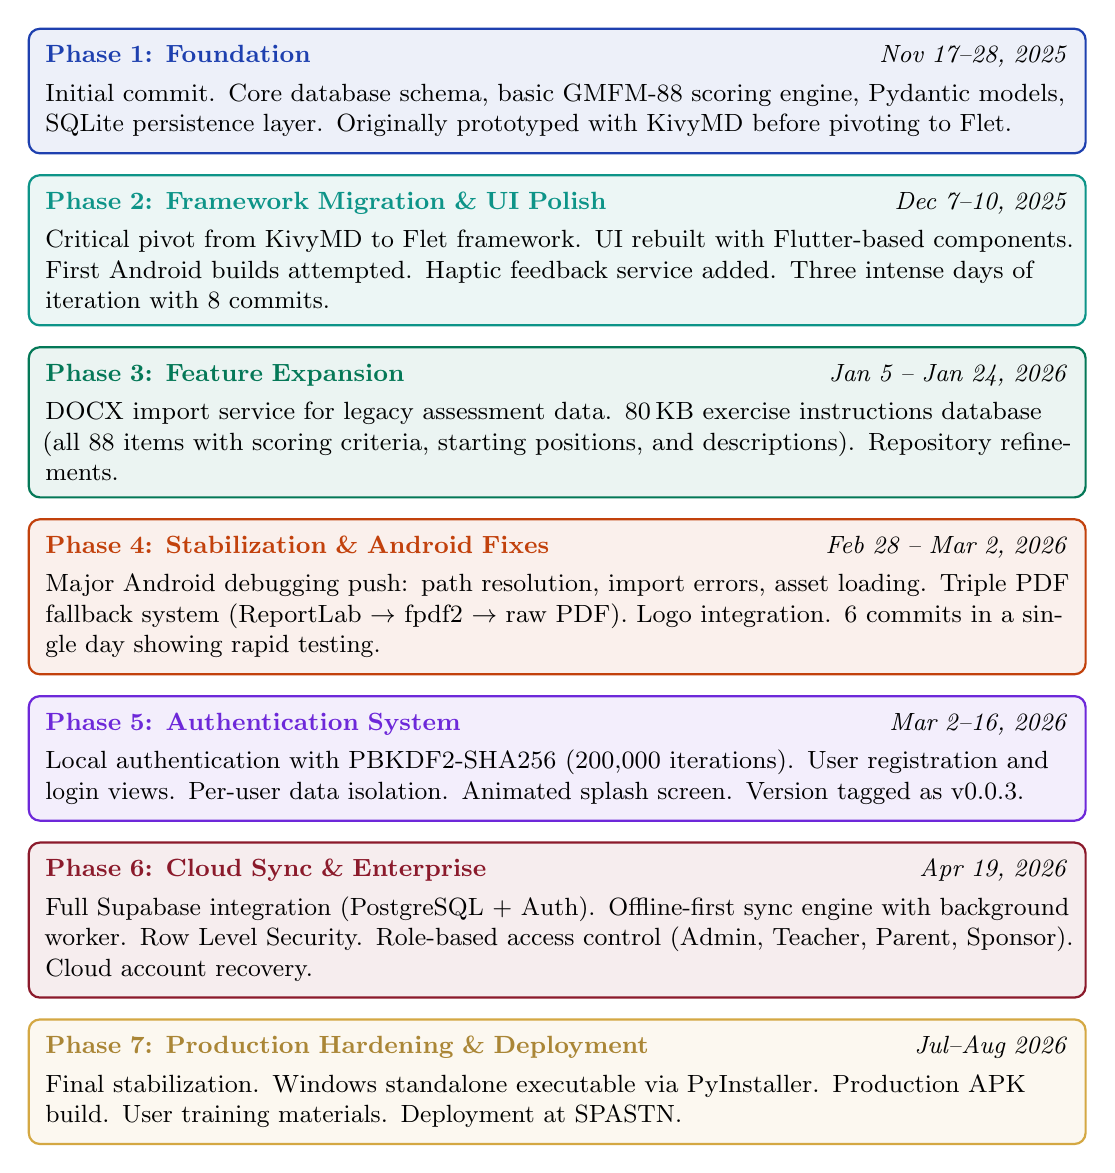
\begin{tikzpicture}[
    node distance=0.1cm,
    phase/.style={
        draw=#1, thick, fill=#1!8,
        rectangle, rounded corners=4pt,
        inner sep=6pt, align=left,
        font=\small, text width=13cm,
    },
    datenode/.style={
        font=\small\bfseries\color{#1},
        anchor=east,
    },
]

\node[phase=visitblue] (p1) {%
    \textbf{\color{visitblue}Phase 1: Foundation} \hfill \textit{Nov 17--28, 2025}\\[3pt]
    Initial commit. Core database schema, basic GMFM-88 scoring engine, Pydantic models, SQLite persistence layer. Originally prototyped with KivyMD before pivoting to Flet.%
};

\node[phase=clinicalteal, below=0.25cm of p1] (p2) {%
    \textbf{\color{clinicalteal}Phase 2: Framework Migration \& UI Polish} \hfill \textit{Dec 7--10, 2025}\\[3pt]
    Critical pivot from KivyMD to Flet framework. UI rebuilt with Flutter-based components. First Android builds attempted. Haptic feedback service added. Three intense days of iteration with 8 commits.%
};

\node[phase=visitgreen, below=0.25cm of p2] (p3) {%
    \textbf{\color{visitgreen}Phase 3: Feature Expansion} \hfill \textit{Jan 5 -- Jan 24, 2026}\\[3pt]
    DOCX import service for legacy assessment data. 80\,KB exercise instructions database (all 88 items with scoring criteria, starting positions, and descriptions). Repository refinements.%
};

\node[phase=visitorange, below=0.25cm of p3] (p4) {%
    \textbf{\color{visitorange}Phase 4: Stabilization \& Android Fixes} \hfill \textit{Feb 28 -- Mar 2, 2026}\\[3pt]
    Major Android debugging push: path resolution, import errors, asset loading. Triple PDF fallback system (ReportLab $\rightarrow$ fpdf2 $\rightarrow$ raw PDF). Logo integration. 6 commits in a single day showing rapid testing.%
};

\node[phase=visitpurple, below=0.25cm of p4] (p5) {%
    \textbf{\color{visitpurple}Phase 5: Authentication System} \hfill \textit{Mar 2--16, 2026}\\[3pt]
    Local authentication with PBKDF2-SHA256 (200,000 iterations). User registration and login views. Per-user data isolation. Animated splash screen. Version tagged as v0.0.3.%
};

\node[phase=sathyamaruby, below=0.25cm of p5] (p6) {%
    \textbf{\color{sathyamaruby}Phase 6: Cloud Sync \& Enterprise} \hfill \textit{Apr 19, 2026}\\[3pt]
    Full Supabase integration (PostgreSQL + Auth). Offline-first sync engine with background worker. Row Level Security. Role-based access control (Admin, Teacher, Parent, Sponsor). Cloud account recovery.%
};

\node[phase=softgold, below=0.25cm of p6] (p7) {%
    \textbf{\color{softgold!80!black}Phase 7: Production Hardening \& Deployment} \hfill \textit{Jul--Aug 2026}\\[3pt]
    Final stabilization. Windows standalone executable via PyInstaller. Production APK build. User training materials. Deployment at SPASTN.%
};

\end{tikzpicture}
\caption*{\small Complete development timeline spanning seven phases across nine months.}
\end{figure}

% ── Git Commit Summary ──────────────────────────────────────────────────────
\subsection{By The Numbers}

\begin{table}[H]
\centering
\renewcommand{\arraystretch}{1.4}
\begin{tabularx}{0.7\textwidth}{X r}
\toprule
\textbf{Metric} & \textbf{Value} \\
\midrule
Total development period                         & 9 months \\
Git commits                                      & 28 \\
Source files (\texttt{.py} + \texttt{.json})     & 34+ \\
Total lines of application code                   & 15,000+ \\
UI views                                          & 6 \\
Backend services                                  & 12 \\
Database tables (local + cloud)                   & 9 \\
Schema migrations                                 & 9 \\
GMFM items digitized                             & 88 \\
Motor domains covered                             & 5 \\
User roles supported                              & 4 \\
PDF generation backends                           & 3 \\
Platforms supported                               & 4 (Android, iOS, Windows, Linux) \\
\bottomrule
\end{tabularx}
\end{table}

% ════════════════════════════════════════════════════════════════════════════
\section{The Application: MotorMeasure Pro}
% ════════════════════════════════════════════════════════════════════════════

\subsection{What Does the App Do?}

\textbf{MotorMeasure Pro} is a cross-platform clinical assessment application that replaces the paper-based GMFM-88 scoring process with a digital workflow. It enables therapists to:

\begin{multicols}{2}
\begin{itemize}[leftmargin=1.5em, itemsep=3pt]
    \item Score all 88 items across 5 motor domains with a tap-based interface
    \item View built-in exercise instructions and scoring criteria for each item
    \item Auto-calculate domain percentages and total scores instantly
    \item Manage patient profiles with encrypted personal data
    \item Track progress over time with session history and trend charts
    \item Generate PDF reports matching the official GMFM scoresheet format
    \item Sync data to the cloud for backup and multi-device access
    \item Import legacy DOCX assessment records
    \item Work entirely offline and sync when connectivity is available
    \item Support multiple user roles (Admin, Therapist, Parent, Sponsor)
\end{itemize}
\end{multicols}

\vspace{0.3cm}
\begin{center}
    \begin{photoplaceholder}[height=7cm, width=0.9\textwidth]
        \vspace{2.5cm}
        {\large\bfseries Application Screenshots}\\[0.3cm]
        {\small Insert a collage of app screenshots showing: Dashboard, Scoring View, PDF Report, Session History}
    \end{photoplaceholder}
\end{center}

\subsection{Technology Stack}

\begin{table}[H]
\centering
\renewcommand{\arraystretch}{1.3}
\begin{tabularx}{\textwidth}{l l X}
\toprule
\textbf{Layer} & \textbf{Technology} & \textbf{Purpose} \\
\midrule
Language         & Python 3.11+                          & Core runtime \\
UI Framework     & Flet (Flutter-based)                  & Cross-platform native rendering \\
Local Database   & SQLite                                & Offline-first data persistence \\
Cloud Backend    & Supabase (PostgreSQL + Auth)           & Cloud sync, authentication, RLS \\
PDF Generation   & fpdf2 / ReportLab / Raw PDF            & Triple-fallback report generation \\
Encryption       & Fernet (cryptography library)          & Field-level encryption at rest \\
Auth             & PBKDF2-SHA256 (200k iterations)        & Secure local password hashing \\
Build            & Flet CLI / PyInstaller                 & Android APK, Windows .exe \\
\bottomrule
\end{tabularx}
\end{table}

\subsection{Architecture Overview}

The application follows a clean \textbf{three-layer architecture}:

\begin{figure}[H]
\centering
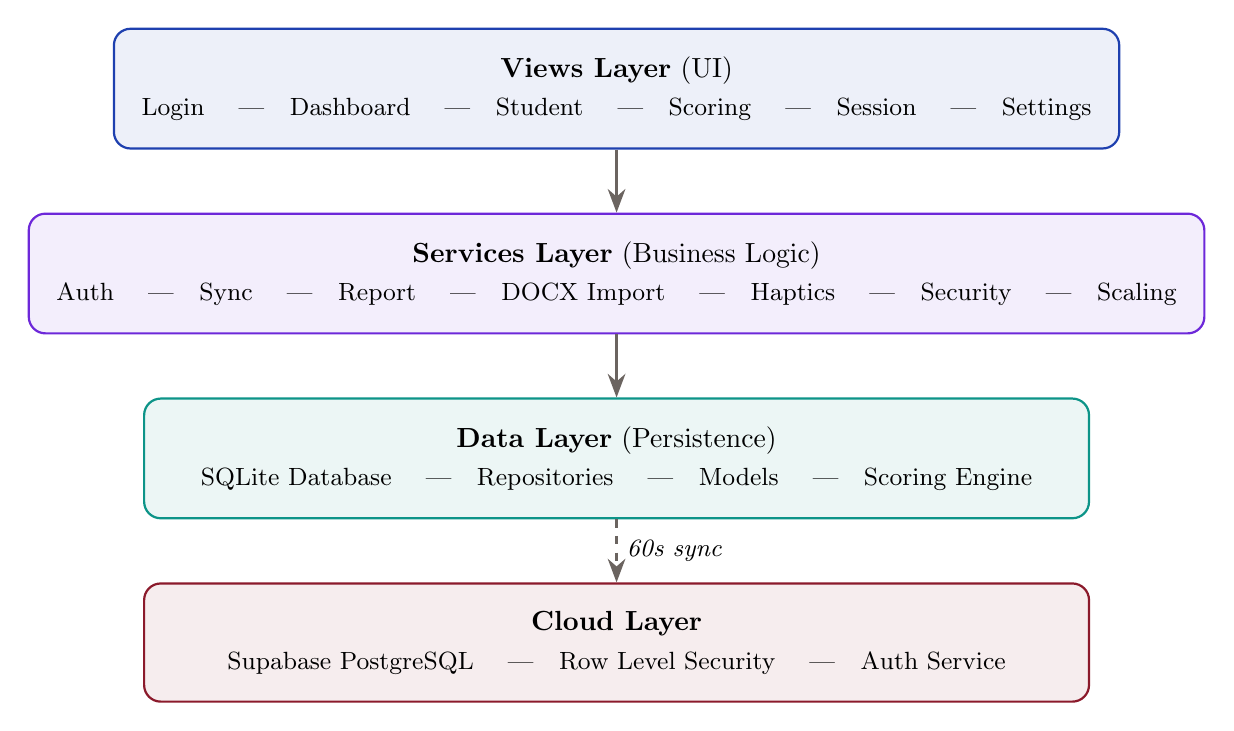
\begin{tikzpicture}[
    node distance=0.6cm,
    layer/.style={
        draw=#1, thick, fill=#1!8,
        rectangle, rounded corners=6pt,
        inner sep=10pt, align=center,
        font=\normalsize, minimum width=12cm, minimum height=1.2cm,
    },
    arrow/.style={-{Stealth[length=3mm]}, thick, draw=warmgray},
]

\node[layer=visitblue] (views) {%
    \textbf{Views Layer} (UI)\\[2pt]
    {\small Login \quad|\quad Dashboard \quad|\quad Student \quad|\quad Scoring \quad|\quad Session \quad|\quad Settings}%
};

\node[layer=visitpurple, below=0.8cm of views] (services) {%
    \textbf{Services Layer} (Business Logic)\\[2pt]
    {\small Auth \quad|\quad Sync \quad|\quad Report \quad|\quad DOCX Import \quad|\quad Haptics \quad|\quad Security \quad|\quad Scaling}%
};

\node[layer=clinicalteal, below=0.8cm of services] (data) {%
    \textbf{Data Layer} (Persistence)\\[2pt]
    {\small SQLite Database \quad|\quad Repositories \quad|\quad Models \quad|\quad Scoring Engine}%
};

\node[layer=sathyamaruby, below=0.8cm of data] (cloud) {%
    \textbf{Cloud Layer}\\[2pt]
    {\small Supabase PostgreSQL \quad|\quad Row Level Security \quad|\quad Auth Service}%
};

\draw[arrow] (views) -- (services);
\draw[arrow] (services) -- (data);
\draw[arrow, dashed] (data) -- node[right, font=\small\itshape] {60s sync} (cloud);

\end{tikzpicture}
\caption*{\small Layered application architecture. Dashed line indicates asynchronous background sync.}
\end{figure}

% ════════════════════════════════════════════════════════════════════════════
\section{Key Challenges \& How We Overcame Them}
% ════════════════════════════════════════════════════════════════════════════

\subsection{Challenge 1: No Problem Statement}

\textbf{The Challenge:} When the EPICS community project was assigned, we had no predefined problem statement. We were simply told to visit a community partner and ``find something useful to build.''

\textbf{How We Overcame It:} We embraced the ambiguity. Our first faculty visit to SPASTN --- where we met the Director and the entire team --- was focused on observation and understanding. We watched, listened, and asked questions. By immersing ourselves in the therapists' daily workflow, the problem emerged naturally. This ``design thinking'' approach taught us that the best solutions come from understanding people, not from textbooks.

\subsection{Challenge 2: Framework Pivot}

\textbf{The Challenge:} Our initial prototype was built using KivyMD, which proved difficult for cross-platform deployment, especially on Android.

\textbf{How We Overcame It:} In early December 2025, we made the difficult decision to migrate to the Flet framework. This required rebuilding the entire UI, but Flet's Flutter-based rendering gave us truly native performance on both Android and desktop. Three intense days of rebuilding saved us months of deployment headaches.

\subsection{Challenge 3: Android Deployment}

\textbf{The Challenge:} Mobile deployment introduced numerous platform-specific issues --- file paths, missing libraries, asset loading failures, and accessibility scaling differences.

\textbf{How We Overcame It:} We implemented multiple compatibility layers:
\begin{itemize}[leftmargin=2em, itemsep=2pt]
    \item Embedded logo assets as base64 to avoid file-path issues
    \item Created a triple PDF fallback system (ReportLab $\rightarrow$ fpdf2 $\rightarrow$ hand-crafted raw PDF)
    \item Built an adaptive UI scaling service that reads Android's accessibility settings
    \item Added lazy imports throughout the codebase for graceful degradation
\end{itemize}

\subsection{Challenge 4: Offline-First with Cloud Sync}

\textbf{The Challenge:} Therapy rooms at SPASTN had unreliable internet. The app needed to work completely offline while still supporting cloud backup when connectivity was available.

\textbf{How We Overcame It:} We designed a git-like sync architecture:
\begin{itemize}[leftmargin=2em, itemsep=2pt]
    \item Every write operation logs to a local \texttt{sync\_queue} table
    \item A background worker thread checks for pending items every 60 seconds
    \item When connectivity is detected, items are pushed to Supabase via REST API
    \item Newer cloud records are pulled and merged into the local database
    \item Local changes always take priority to prevent data loss
\end{itemize}

\subsection{Challenge 5: Clinical Data Privacy}

\textbf{The Challenge:} Patient data --- especially names and identifiers of children with disabilities --- required strict privacy protection.

\textbf{How We Overcame It:} We implemented multiple layers of security:
\begin{itemize}[leftmargin=2em, itemsep=2pt]
    \item Field-level Fernet encryption for patient names and identifiers at rest
    \item PBKDF2-SHA256 password hashing with 200,000 iterations
    \item Row Level Security on the cloud database (each user sees only their own data)
    \item Role-based access control with four distinct permission levels
\end{itemize}

% ════════════════════════════════════════════════════════════════════════════
\section{Impact \& Outcomes}
% ════════════════════════════════════════════════════════════════════════════

\begin{highlightbox}[Project Impact at a Glance]
\begin{multicols}{2}
\begin{itemize}[leftmargin=1.5em, itemsep=4pt]
    \item[\color{clinicalteal}\textbf{$\downarrow$}] \textbf{40\% reduction} in assessment paperwork time
    \item[\color{clinicalteal}\textbf{$\uparrow$}] \textbf{100\% elimination} of manual calculation errors
    \item[\color{clinicalteal}\textbf{$\uparrow$}] \textbf{Instant PDF reports} generated in one tap
    \item[\color{clinicalteal}\textbf{$\uparrow$}] \textbf{Longitudinal tracking} of child progress over months and years
    \item[\color{clinicalteal}\textbf{$\uparrow$}] \textbf{Secure cloud backup} of all patient data
    \item[\color{clinicalteal}\textbf{$\uparrow$}] \textbf{Multi-device access} for therapists
\end{itemize}
\end{multicols}
\end{highlightbox}

\subsection{For the Therapists}

The application directly addresses the pain points identified during our first visit:
\begin{itemize}[leftmargin=2em]
    \item \textbf{Time savings:} What took 20--30 minutes on paper now takes under 10 minutes digitally
    \item \textbf{Accuracy:} Auto-calculated domain percentages and total scores eliminate arithmetic errors
    \item \textbf{Accessibility:} In-app exercise instructions mean therapists don't need to refer to separate manuals
    \item \textbf{Continuity:} Cloud sync ensures data is never lost, even if a device is damaged
\end{itemize}

\subsection{For the Children \& Parents}

\begin{itemize}[leftmargin=2em]
    \item \textbf{Better therapy planning:} With accurate progress tracking, therapists can tailor programs to each child's needs
    \item \textbf{Clear progress reports:} Parents receive professional PDF reports showing their child's improvement
    \item \textbf{More therapy time:} Less time spent on paperwork means more time spent with each child
\end{itemize}

\subsection{For the Institution}

\begin{itemize}[leftmargin=2em]
    \item \textbf{Real-world learning:} Students gained hands-on experience in requirement gathering, app development, testing, and deployment with an NGO through the EPICS community project framework
    \item \textbf{Sustainable technology transfer:} A complete, maintainable solution was delivered that SPASTN can continue using independently
    \item \textbf{EPICS community impact:} Demonstrates Sathyabama's commitment to using engineering and technology for social welfare through community service
\end{itemize}

% ════════════════════════════════════════════════════════════════════════════
\section{Official App Release}
% ════════════════════════════════════════════════════════════════════════════

The \textbf{MotorMeasure Pro} application was officially released under the auspices of our \textbf{Hon'ble Chancellor, Dr. Mariazeena Johnson}, marking the successful culmination of our EPICS community project and the transition of a student initiative into a deployed, real-world clinical tool.

\begin{minipage}{0.48\textwidth}
    \begin{photoplaceholder}[height=5cm]
        \vspace{1.5cm}
        {\small\bfseries Chancellor Releasing the App}\\[0.2cm]
        {\footnotesize Photo of Dr. Mariazeena Johnson releasing the app}
    \end{photoplaceholder}
\end{minipage}
\hfill
\begin{minipage}{0.48\textwidth}
    \begin{photoplaceholder}[height=5cm]
        \vspace{1.5cm}
        {\small\bfseries Team with Chancellor}\\[0.2cm]
        {\footnotesize Photo of the team with the Chancellor}
    \end{photoplaceholder}
\end{minipage}

% ════════════════════════════════════════════════════════════════════════════
\section{Acknowledgements}
% ════════════════════════════════════════════════════════════════════════════

We express our deepest gratitude to the following individuals and institutions whose support made this EPICS community project possible:

\begin{itemize}[leftmargin=2em, itemsep=4pt]
    \item \textbf{Hon'ble Chancellor Dr. Mariazeena Johnson} --- for her constant support, encouragement, and for officially releasing the application
    \item \textbf{Dr. P. Sarasu} (Dean) --- for providing institutional support and resources
    \item \textbf{Dr. Minu Susan Jacob} (Faculty Guide) --- for continuous mentorship, coordination, and accompanying the team on our inaugural faculty visit to SPASTN
    \item \textbf{The Director of SPASTN} --- for endorsing our EPICS community project and providing full organizational support
    \item \textbf{Ms. Jemima} (Principal, SPASTN) --- for welcoming us and facilitating our visits
    \item \textbf{The Physiotherapists at SPASTN} --- for their patience, feedback, and willingness to adopt new technology
    \item \textbf{The Children and Families at SPASTN} --- whose resilience and strength inspired every line of code we wrote
    \item \textbf{Sathyabama Institute of Science and Technology} --- for providing the resources, platform, and vision to pursue the EPICS community project for social impact
\end{itemize}

\vspace{0.5cm}

\begin{quotecallout}
``The GMFM-88 was developed by Dianne Russell, Peter Rosenbaum, and colleagues at the CanChild Centre for Childhood Disability Research, McMaster University. We gratefully acknowledge their foundational work that made this application possible.''
\end{quotecallout}

% ════════════════════════════════════════════════════════════════════════════
\section{Looking Ahead}
% ════════════════════════════════════════════════════════════════════════════

While the current release represents a fully functional and deployed solution, we envision several future enhancements:

\begin{itemize}[leftmargin=2em, itemsep=3pt]
    \item \textbf{GMFCS Classification Integration} --- Adding the Gross Motor Function Classification System to complement GMFM scoring
    \item \textbf{GMFM-66 Scale Support} --- Implementing item difficulty lookup tables for the 66-item scale
    \item \textbf{Video-Assisted Scoring} --- Allowing therapists to record and annotate assessment videos
    \item \textbf{Multi-Center Dashboard} --- Aggregate analytics across all SPASTN centers
    \item \textbf{Parent Portal} --- A dedicated interface for parents to view their child's progress
    \item \textbf{Deployment to Additional Centers} --- Expanding to SPASTN's Washermanpet and Ayanavaram locations
\end{itemize}

\vspace{1cm}

% ── Closing ─────────────────────────────────────────────────────────────────

\begin{center}
{\color{sathyamaruby}\rule{0.3\textwidth}{1pt}}\\[0.5cm]
{\large\color{deepnavy}\textit{``Technology finds its highest purpose when it serves those who need it most.''}}\\[0.8cm]

{\small\color{warmgray} Department of Computer Science and Engineering}\\
{\small\color{warmgray} Sathyabama Institute of Science and Technology}\\
{\small\color{warmgray} Jeppiaar Nagar, Rajiv Gandhi Salai, Chennai -- 600119}\\[0.3cm]
{\small\color{warmgray} Academic Year 2025--2026}\\[0.5cm]
{\color{sathyamaruby}\rule{0.3\textwidth}{1pt}}
\end{center}

% ============================================================================
\end{document}
